\chapter{Experimental Approach} \label{ch_eva} % Or alternatives

Once presented the problem and a proposed methodology to treat it, some approach is required to test the feasibility of the ideas.
With this in mind, and given the practical interest of the problem, an experimental approach is proposed, using the library example (section \ref{sec_Library}) as a testing case to implement and analyse the proposed ideas. 
The library setting is flexible enough to be stated with different degrees of complexity and putting special emphasis on critical areas (e.g. temporal analysis, incomplete information, etc.).

%In this case, the proposed experimental environment is the library setting described in section \ref{sec_Library} with some simplifications and extensions to emphasize particular parts of the problem.
%By these means, the problem can be divided in smaller

\section{Library Example}

The library setting, presented in section \ref{sec_Library}, provides a good testing environment.
It has some desired qualities for experimentation, principally, a bounded space and a compact set of activities.
%Now, some incremental

Let first introduce a simplified version of the library setting.
%If we reuse the library example from chapter 1 it is worth to show how the presented approach applies to that problem.
%With this in mind, let's first make a simplification of the example.
In Figure \ref{fig:ex_library} is presented a \textit{linear} library. 
It has five connected and consecutive regions: (A) main entrance, (B) printing area, (C) reception, (D) bookshelf and (E) common area.

\begin{figure}[h]
\centering
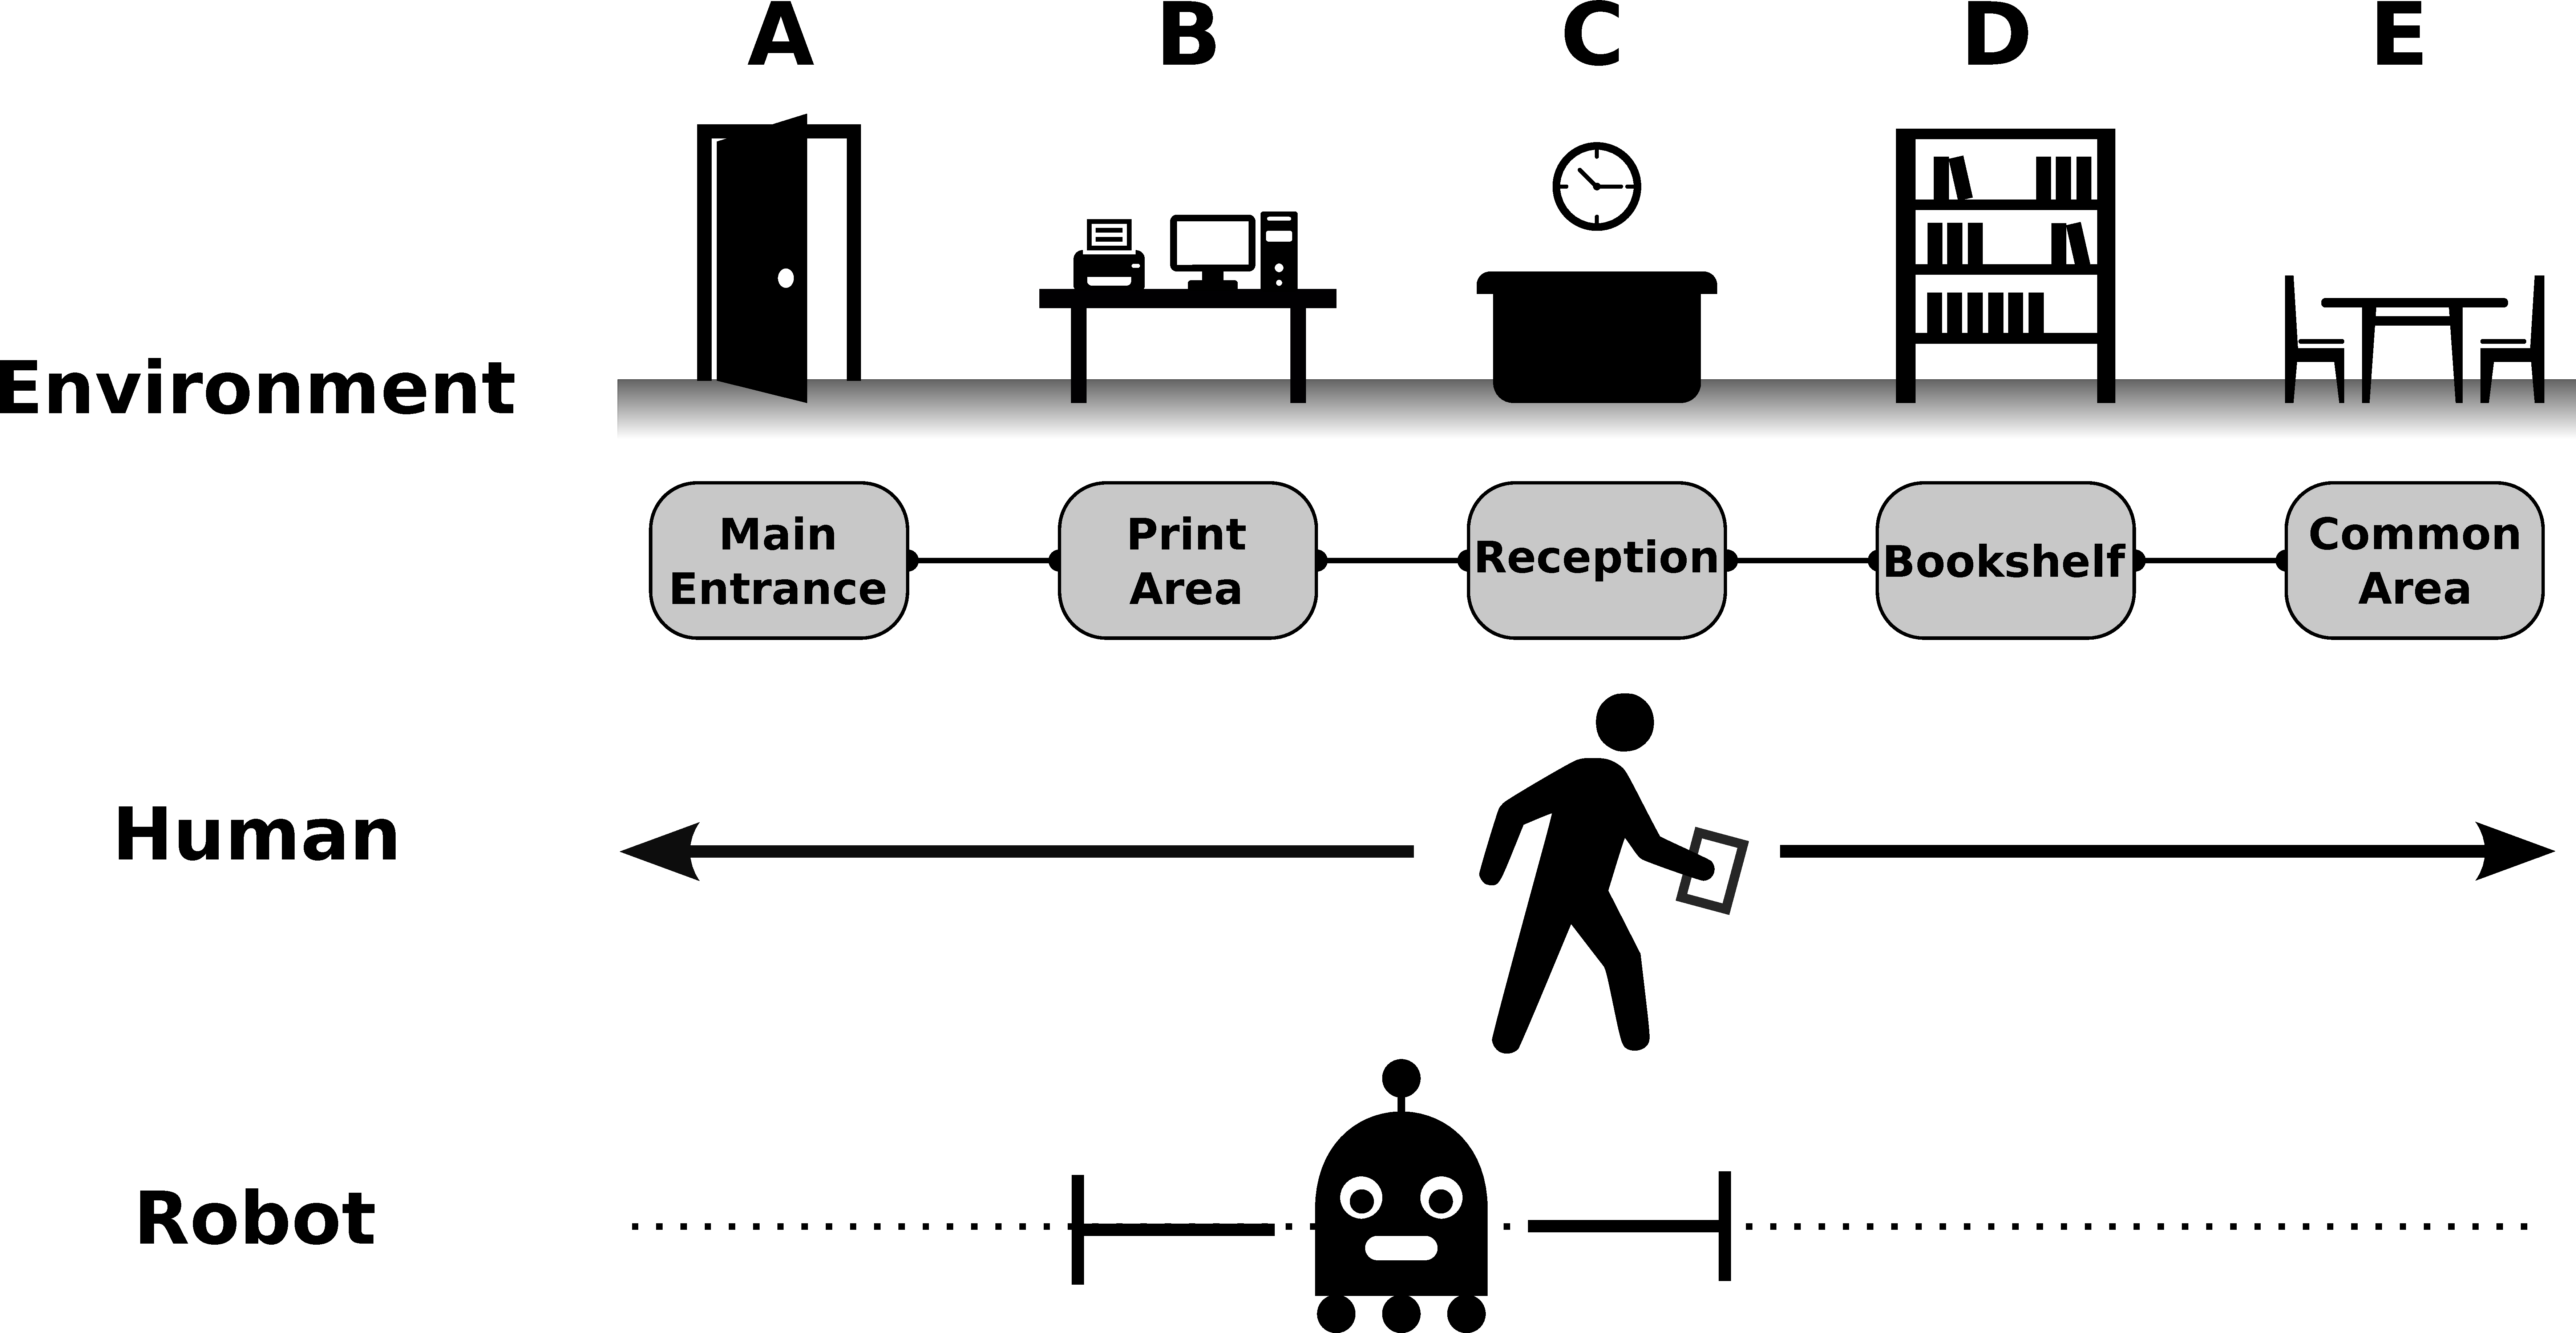
\includegraphics[width=\textwidth]{fig/ex_library.pdf}
\caption{Simplified library setting}
\label{fig:ex_library}
\end{figure}


In this simplified world a person and a robot can move linearly to any region, and they don't obstruct each other.
An activity is performed by a person by visiting regions in a proper order and spending \textit{enough} time on each of them, these intervals are considered within the activity representation.
The challenge here is to recognize the activities of the person.
The robot have an active role by tracking and following the human through the regions he visits and labelling this within its internal world model.

The following activities can be defined:

\begin{description}
\item[print]$B$ 
\item[study]$D \rightarrow E \rightarrow D$
\item[bookLoan]$D \rightarrow C$
\item[bookRetrieval]$C$
\item[requestAssistance]$C$
\end{description}

Now the problem is, given a particular state of the world, to recognize the ongoing activity.
The representations can complete by considering all the occurring states for an activity, but in reality, a robot can realize about the activity in when an intermediate state is occurring. For example, the robot may be watching someone standing in front of the Bookshelf (region $D$), at this point there are two possible activities to consider: \textit{bookLoan} or \textit{study}, because $D$ is an ambiguous state. In this case, the future state will decide the activity.

Now, some extensions can be induced to this simplified world.
\begin{itemize}
\item A robot can have limited sensors, so it will only be able to sense two regions at the same time. 
So, some activeness is required. For example, being observed a person going towards the common area, the robot can move to confirm the position of the person.
\item Handling multiple subjects in the scene, complicates the problem. The robot won't be able to observe all of them, but may try to maximize the observations and after labelling some individuals may go back and sense the rest of the subjects.
\item Object recognition can be induced to disambiguate activities. For example, two activities with the same region description can have an additional parameter regarding the presence of an object. In these cases, a robot can go an confirm the presence or absence of the object to discriminate its hypotheses. 
\end{itemize} 

\subsection{Experimental stages}

Four different stages of the library setting are presented that enables progressive analysis and testing of the ideas within this project. These stages goes from simplistic simulations towards a real robotic platform performing activity recognition, which is the ultimate goal of the research in this project.


\subsubsection{Terminal Simulation}
An implementation of the library setting in as a \textit{terminal} simulation.
The activity representations are defined explicitly and the world states can be defined explicitly as well, or generated with another program.
\begin{itemize}
\item[Pros:]
\item Simplicity
\item Flexible to rapidly implement different cases
\item Simple agents (humans and robot) can be modelled.
\item Controllable parameters
\item Repeatability
\end{itemize}
\begin{itemize}
\item[Cons:]
\item Non realistic data
\end{itemize}

\subsubsection{MORSE Simulation}
MORSE is a simulation environment designed explicitly for robotics which allows compatibility of between the simulation environment and real robotic platforms. An implementation a 3D robotic simulator would enable to test more realistic cases which also can be repeated to test different approaches. Robots, human avatars and sensors are available to be controlled and to retrieve data. 

\begin{itemize}
\item[Pros:]
\item Robotic oriented environment
\item More realistic representations of activities
\item Controllable parameters
\item Repeatability
\item Straight forward software integration
\end{itemize}
\begin{itemize}
\item[Cons:]
\item Non realistic data
\item Integration takes time
\end{itemize}


\subsubsection{Dataset Analysis}
Datasets for activity recognition are available (see \citep{Tenorth2009_TUMKData,Liu2011_BenchmarkDatasHAR}). They provide a standardized test bed for different techniques. While it would difficult to find datasets that take in consideration a robotic platform, it is worth to test individual parts of the overall system to compare with other approaches.
\begin{itemize}
\item[Pros:]
\item Standard data test bed and benchmarking
\item Results available for comparison
\item Repeatability
\end{itemize}
\begin{itemize}
\item[Cons:]
\item Analysis \textit{a posteriori}
\item No robot present, so no active behaviour would be possible
\item Data relies on specific conditions
\end{itemize}

\subsubsection{Robot}
The end goal of this project is to provide robots with the capacity to recognize human activities and understand the relation between them and the environment. This goal far beyond the scope of this project. However, experimentation with real robotic systems is an important step in that direction as real environment conditions are difficult to replicate, and also because the application of these king of systems is oriented mostly in this direction.
\begin{itemize}
\item[Pros:]
\item Real conditions
\item New problems can emerge from non considered situations
\end{itemize}
\begin{itemize}
\item[Cons:]
\item Difficult repeatability
\item Dynamic and non deterministic environment
\item Difficult implementation and slow experimentation
\item Noisy and Uncertain data
\end{itemize}


%TODO %TODO %TODO Complete the example.











% Main parts of the problem

% A - Scene decomposition (locations, objects, persons)
%   > from observations to scene reconstruction

% B - 

% B - Representation 
% Modelling in space (QSR)
% Modelling in time (QSTR)











